\section{CDMA (code division multiple access)}
The idea behind this system is that all transmitters use the same time and frequency allocation. To distinguish the different users, a code is assigned to each of them. The code is then used to spread a small information bandwidth over the much wider channel bandwidth. CDMA is thus a spread spectrum (FH-SS) technique. There are two ways to do that, one is frequency hopping (FH-SS) and the other is by  multiplying the data sequence with a much higher chip sequence (DSSS), as one can see in \autoref{fig:dsss}.
\begin{figure}[ht]
  \centering
  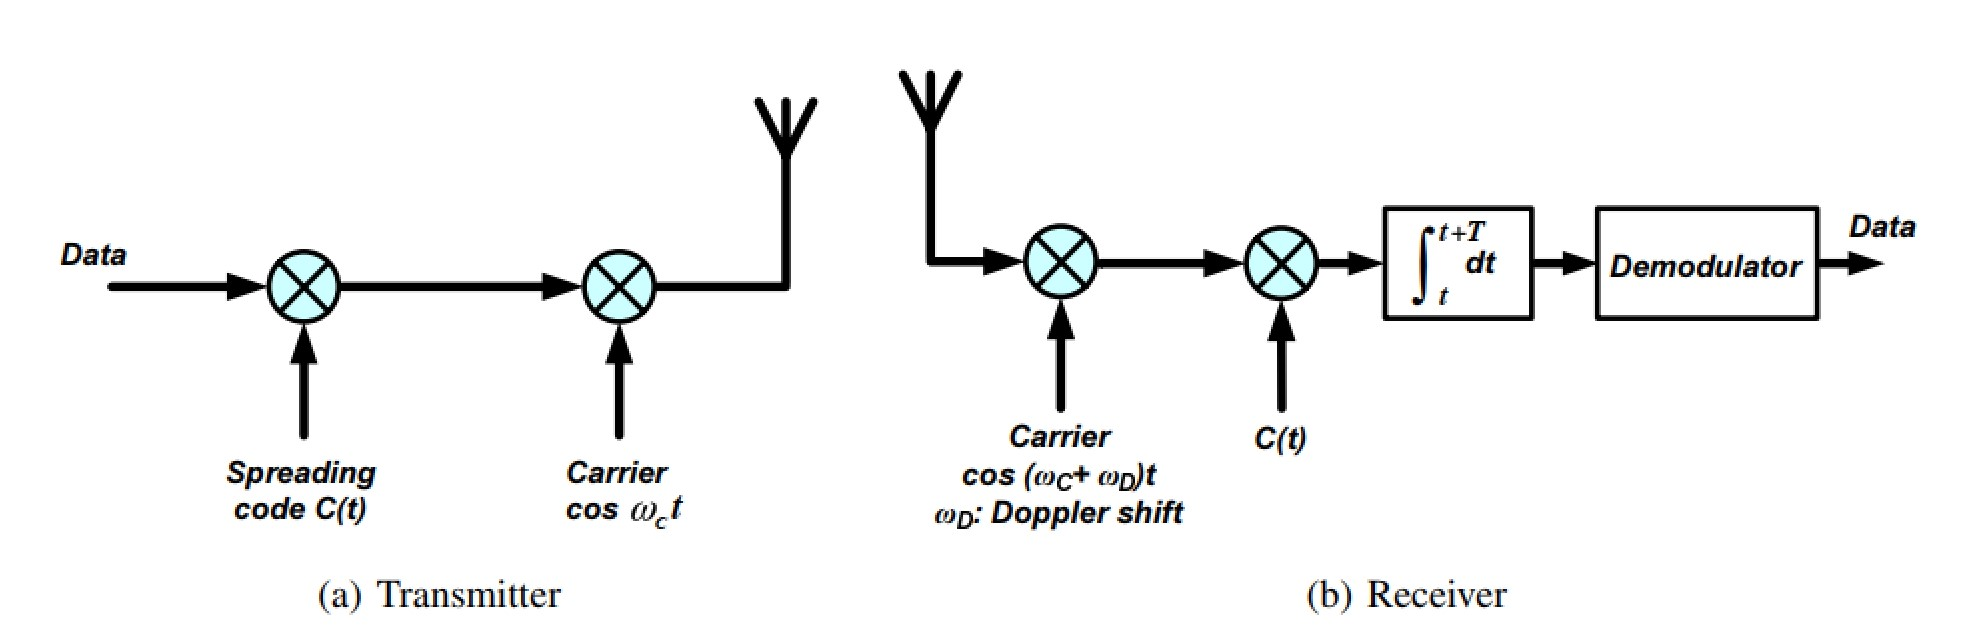
\includegraphics[width=13cm]{images/spread_spectrum_tx_rx.jpg}
  \caption{Spread Sepctrum}
  \label{fig:dsss}
\end{figure}
The spreading gain of such a system can be calculated according to \autoref{eq:spreading_gain}, where the bit time is called $T_d$ and the chip time $T_c$.
\begin{equation}\label{eq:spreading_gain}
G_{\mathrm{dB}}=10 \log _{10} \frac{\mathrm{SNR}_{\text {out }}}{\mathrm{SNR}_{\text {in }}}=10 \log _{10} \frac{B_{\mathrm{ss}}}{B_{\mathrm{d}}}=10 \log _{10} \frac{T_{\mathrm{d}}}{T_{\mathrm{c}}}
\end{equation}
\subsubsection{Shor Summary}
CDMA (Code Division Multiple Access) is a wireless communication technology that uses unique codes to separate different signals in the same frequency band. It was mainly used in some areas for 2G and 3G cellular network technology.

Spreading is the process of assigning a unique code to each user's data to distinguish it from other users' data. The receiver then applies the same code to decode the intended data (For that one uses the m-sequences (Glonass), Gold codes (e.g. GPS)). Spreading allows multiple users to share the same frequency band simultaneously by separating their signals through code division. This results in an increase in the number of users that can access the network and improves the overall network capacity. (When doing this, one increases the bandwidth (frequency))
\subsection{UMTS (Universal Mobile Telecommunications System)}
Is the most prominent communication system in Europe. As opposed to GSM and other TDMA-based cellular systems, where one user has a link to one cell only at one given time, a UTMS user can use signals from two base stations. They send with the same user code, such that the signal looks as if it was sent through a multipath environment. Thus, we do not have a hard handover when changing from one cell to another, but rather a smooth, so-called soft handover, where the user may have a simultaneous link to two base stations during a transition phase
\subsection{Hadamard matrix / Walsh matrices}
Hadamard matrix / Walsh matrices are used to generate the code for the different users in a system as it can also be seen in \autoref{subsubsec:example_cdma}.
The equation to calculate the Hadamard matrix can be found in \autoref{eq:hadamard}. To do the calculation one must know the Kronecker Product ($\otimes$) to which an example can be found in \autoref{eq:kronecker_example}. An important property of the Hadamard matrix is that when one multiplies two rows with each other and ads them up the result is always zero see also \autoref{eq:hardamard_test}. In the end one multiplies the signal for a certain user with one column of the matrix. The receiver (user) does the same and is then able to decode the signal.
\begin{equation} \label{eq:hadamard}
\begin{aligned}
&H_1=[1],\\
&H_2=\left[\begin{array}{cc}
1 & 1 \\
1 & -1
\end{array}\right] \text {, }\\
&H_4=\left[\begin{array}{cccc}
1 & 1 & 1 & 1 \\
1 & -1 & 1 & -1 \\
1 & 1 & -1 & -1 \\
1 & -1 & -1 & 1
\end{array}\right]\\
&H_{2^k}=\left[\begin{array}{cc}
H_{2^{k-1}} & H_{2^{k-1}} \\
H_{2^{k-1}} & -H_{2^{k-1}}
\end{array}\right]=H_2 \otimes H_{2^{k-1}}
\end{aligned}
\end{equation}
\subsubsection{Kronecker Product}
\begin{equation}\label{eq:kronecker_example}
\left[\begin{array}{ll}
1 & 2 \\
3 & 4
\end{array}\right] \otimes\left[\begin{array}{ll}
0 & 5 \\
6 & 7
\end{array}\right]-\left[\begin{array}{llll}
1 \cdot 0 & 1 \cdot 5 & 2 \cdot 0 & 2 \cdot 5 \\
1 \cdot 6 & 1 \cdot 7 & 2 \cdot 6 & 2 \cdot 7 \\
3 \cdot 0 & 3 \cdot 5 & 4 \cdot 0 & 4 \cdot 5 \\
3 \cdot 6 & 3 \cdot 7 & 4 \cdot 6 & 4 \cdot 7
\end{array}\right]-\left[\begin{array}{cccc}
0 & 5 & 0 & 10 \\
6 & 7 & 12 & 14 \\
0 & 15 & 0 & 20 \\
18 & 21 & 24 & 28
\end{array}\right]
\end{equation}
\subsubsection{carrier-to-interference ratio (C/I)}
The carrier-to-interference ratio (C/I) in CDMA refers to the ratio of the power of the desired signal to the power of the unwanted interference in the system. A higher C/I ratio indicates a better signal quality and a lower level of interference, which can result in improved system performance and capacity. For example a carrier-to-interference ratio (C/I) of 1000 means that the power of the desired signal is 1000 times greater than the power of the unwanted interference. This indicates that the signal quality is very good and there is a low level of interference in the system. A high C/I ratio is desirable in CDMA communication systems as it results in improved system performance and capacity. A C/I ratio of 1000 is considered very high and provides excellent signal quality and minimal interference.
\subsubsection{Exercise calculate hadamard matrix}
Construct the Hadamard matrix $H_8$ and check the orthogonality property of the codes given by row 2 and row 8, respectively.
$$
H_8=\left[\begin{array}{cccccccc}
1 & 1 & 1 & 1 & 1 & 1 & 1 & 1 \\
1 & -1 & 1 & -1 & 1 & -1 & 1 & -1 \\
1 & 1 & -1 & -1 & 1 & 1 & -1 & -1 \\
1 & -1 & -1 & 1 & 1 & -1 & -1 & 1 \\
1 & 1 & 1 & 1 & -1 & -1 & -1 & -1 \\
1 & -1 & 1 & -1 & -1 & 1 & -1 & 1 \\
1 & 1 & -1 & -1 & -1 & -1 & 1 & 1 \\
1 & -1 & -1 & 1 & -1 & 1 & 1 & -1
\end{array}\right]
$$
\begin{equation}\label{eq:hardamard_test}
\begin{aligned}
H_{8_2} \cdot H_{8_8}^T & =\left[\begin{array}{llllllll}
1 & -1 & 1 & -1 & 1 & -1 & 1 & -1
\end{array}\right] \cdot\left[\begin{array}{llllllll}
1 & -1 & -1 & 1 & -1 & 1 & 1 & -1
\end{array}\right]^T \\
& =1+1-1-1-1-1+1+1=0 .
\end{aligned}
\end{equation}
\subsubsection{Exercise CDMA}
Now let us assume a CDMA system with a data rate of 125 kbit/s (BPSK with a $\pm $1 data stream), a chip rate of 1 Mchip/s and a carrier frequency of $f_c$. Sketch the transmitter of such a system and assign important parameters.
\paragraph{Sketch the receiver of such a system and assign important parameters.}\mbox{} \newline
See \autoref{fig:dsss}
\paragraph{Sketch the receiver of such a system and assign important parameters.}\mbox{} \newline
See \autoref{fig:dsss}
\paragraph{Draw in a qualitative way the amplitude spectrum around the RF carrier of the RF signal with only data modulated (no spreading).}\mbox{} \newline
Since the pulse duration is \SI{8e-6}{\second} and the Fourier transform of a rectangle is $|T| \cdot \operatorname{si}(\pi T f)=\SI{8e-6}{}\frac{sin(\SI{8e-6}{\second} \cdot \pi \cdot f)}{\pi \cdot \SI{8e-6}{\second}}$ one can draw the graph. Important to know is that when one solves the following equations$\frac{sin(\SI{8e-6}{\second} \cdot \pi \cdot f)}{\pi \cdot \SI{8e-6}{\second}}=0 \Rightarrow \SI{8e-6}{\second} \cdot \pi \cdot f=\pi$ one gets \SI{125e3}{\hertz} which is half of the null to null bandwidth $\Rightarrow$ the null to null bandwidth is \SI{250e3}{\hertz}, see \autoref{fig:amp_spec1}.
\begin{figure}[ht!]
  \centering
  \resizebox{12cm}{!}{\subimport{images/}{amplitude_spectrum_1.tex}}
  \caption{Amplitude Spectrum}
  \label{fig:amp_spec1}
\end{figure}
\paragraph{Draw in a qualitative way the amplitude spectrum around the RF carrier of the spread RF signal}\mbox{} \newline
Since the pulse duration is \SI{1e-6}{\second} and the Fourier transform of a rectangle is $|T| \cdot \operatorname{si}(\pi T f)=\SI{1e-6}{}\frac{sin(\SI{1e-6}{\second} \cdot \pi \cdot f)}{\pi \cdot \SI{1e-6}{\second}}$ one can draw the graph. Important to know is that when one solves the following equations$\frac{sin(\SI{1e-6}{\second} \cdot \pi \cdot f)}{\pi \cdot \SI{1e-6}{\second}}=0 \Rightarrow \SI{1e-6}{\second} \cdot \pi \cdot f=\pi$ one gets \SI{1e6}{\hertz} which is half of the null to null bandwidth $\Rightarrow$ the null to null bandwidth is \SI{2e6}{\hertz},see \autoref{fig:amp_spec2}.
\begin{figure}[ht!]
  \centering
  \resizebox{12cm}{!}{\subimport{images/}{amplitude_spectrum_2.tex}}
  \caption{Amplitude Spectrum}
  \label{fig:amp_spec2}
\end{figure}
\paragraph{What is the spreading gain}\mbox{} \newline
According to \autoref{eq:spreading_gain} it is $G_{\mathrm{dB}}=10 \log _{10} \frac{T_{\mathrm{d}}}{T_{\mathrm{c}}}=10 \log _{10} \frac{\SI{8e-6}{\second}}{\SI{1e-6}{\second}} \approx 9dB$. The spreading factor would be 8 since the frequency was increased by 8. But this also means the power density maximum has decreased by a factor of 9dB.
\subsubsection{Example 1} \label{subsubsec:example_cdma}
Walsh code should be used with a spreading factor of four and two users should use the channel at the same time. We know from \autoref{eq:hadamard} that with a spreading factor of four we get the following matrix\footnote{\href{https://youtu.be/L4Gvu3gQ0wg}{Video}}:
$$
H_4=\left[\begin{array}{cccc}
\rowcolor{red!20}
1 & 1 & 1 & 1 \\
\rowcolor{green!20}
1 & -1 & 1 & -1 \\
1 & 1 & -1 & -1 \\
1 & -1 & -1 & 1
\end{array}\right]\\
$$
One now has to assign to each user one code. Let's say \colorbox{red!20}{user one} has row one and \colorbox{green!20}{user two} row two. The other rows are inactive. \newline
Let's assume the Data of the users are the following: 
$$
\begin{array}{cccc}
\rowcolor{red!20}
\text{User}_1 & 110010 \\
\rowcolor{green!20}
\text{User}_2 & 001001
\end{array}
$$
This gives then the following \colorbox{blue!20}{code sequence}:\newline
\resizebox{1\textwidth}{!}{$\displaystyle
\begin{array}{llllllllllllllllllllllllll}
\rowcolor{red!20}
1&1&1&1&\mid1&1&1&1&\mid-1&-1&-1&-1&\mid-1&-1&-1&-1&\mid1&1&1&1& \mid-1&-1&-1&-1& \\
\rowcolor{green!20}
-1&1&-1&1&\mid-1&1&-1&1&\mid 1&-1&1&-1&\mid-1&1&-1&1&\mid-1&1&-1&1& \mid 1&-1&1&-1& \\
\rowcolor{blue!20}
0&2&0&2&\mid0&2&0&2&\mid0&-2&0&-2&\mid-2&0&-2&0&\mid0&2&0&2&\mid 0&-2&0&-2&
\end{array}
$}
The receiver does then a sequence wise multiplication with the received data and the assigned walsh-code, which is for user one 1111.\newline
\resizebox{1\textwidth}{!}{$\displaystyle
\begin{array}{llllllllllllllllllllllllll}
\rowcolor{blue!20}
0&2&0&2&\mid0&2&0&2&\mid0&-2&0&-2&\mid-2&0&-2&0&\mid0&2&0&2&\mid 0&-2&0&-2&\\
\rowcolor{red!20}
&&4&&\mid&&4&&\mid&&-4&&\mid&&-4&&\mid&&4&& \mid&&-4&& \\
\end{array}
$}
As one can see from the result above one gets the exact same data as one has transmitted.
\subsection{Frequency hopping}
We do frequency hopping so that if we have interference on a certain frequency, for example from a microwave, one can still receive and send data some data and not all is lost, but only some. To do this the transmitter and receiver are hopping in the same rhythm from one frequency to the other. Fast FHSS (Frequency hopping spread spectrum) means that one bit gets transmitted over multiple frequencies is not used, because one would need to switch the frequency very fast. Slow FHSS each bit gets transmitted over one frequency $\Rightarrow$ Hamming can be used to reconstruct false ones.

\paragraph{What is spreading gain?}\mbox{} \newline
See \autoref{eq:spreading_gain}
\paragraph{What is cell breathing?}\mbox{} \newline
In CDMA-based Cellular networks, cell breathing is a mechanism which allows overloaded cells to offload subscriber traffic to neighbouring cells by changing the geographic size of their service area. Heavily loaded cells decrease in size while neighbouring cells increase their service area to compensate. Thus, some traffic is handed off from the overloaded cell to neighbouring cells, resulting in load balancing.
\subsubsection{Excercise SNR vs. C/I in a CDMA system}
The signal-to-noise ratio given by thermal noise is usually designated as SNR. The corresponding signal-tonoise ratio due to interference by other users on the same channel is described by C/I (carrier-to-interference ratio).\newline
Now consider the following situation. A certain CDMA system can live with an SNR of 10 dB, if no additional
interference is present.
\begin{enumerate}
    \item \textbf{How much would you have to amplify the transmitter power in order to reach an SNR of 13 dB?}\newline
    By a factor of two, because 3db ($10^{\frac{3}{10}}=2$).
    \item \textbf{If spreading codes can be chosen such that a concurrent transmitter produces a C/I of 1000/1, how many transmitters can transmit simultaneously if the total signal-to-noise-plus-interference-ratio SINR is not to fall below the original 10 dB? The SINR is given by the linear measure}
    $$
    \frac{1}{\mathrm{SINR}}=\frac{1}{\mathrm{SNR}}+\frac{1}{C / I}
    $$
    SINR stands for Signal-to-Interference-plus-Noise Ratio in CDMA. It is a measure of the quality of a received signal compared to the combined power of all other interference signals and background noise. A high SINR indicates a strong signal and low interference and noise, while a low SINR indicates weak signal quality and high levels of interference and noise. SINR is an important performance metric in CDMA communication systems as it directly impacts the ability to accurately recover the intended signal. A high SINR results in improved system performance and capacity, while a low SINR can lead to errors and degradation of system performance.
    \item  \textbf{Can you allow more simultaneous transmitters for the same SINR by increasing all transmitter powers?
    $$
    \begin{aligned}
    \frac{1}{\frac{S}{I+N}}=\frac{1}{\text { SINR }} & =\frac{1}{\mathrm{SNR}}+\frac{1}{C / I} \\
    \frac{1}{10} & =\frac{1}{20}+\frac{1}{20} \\
    C / I & =13 \mathrm{~dB}=20 \\
    n \cdot \frac{1}{1000} & =\frac{1}{20} \Rightarrow n=\underline{50}
    \end{aligned}
    $$
Where are the limits?}\newline
\end{enumerate}
\subsection{M-Sequences}
Maximum-length sequences have very interesting autocorrelation properties: they have one peak for exact alignment, and the same low level for misalignment of one or more chips.
\begin{equation}
\begin{array}{ccc}
\hline \text { Degree }(L) & \text { Sequence length }\left(N=2^L-1\right) & \text { Primitive polynomial } \\
\hline 1 & 1 & x+1 \\
2 & 3 & x^2+x+1 \\
3 & 7 & x^3+x+1 \\
4 & 15 & x^4+x+1 \\
5 & 31 & x^5+x^2+1 \\
6 & 63 & x^6+x+1 \\
7 & 127 & x^7+x+1 \\
8 & 255 & x^8+x^7+x^2+x+1 \\
9 & 511 & x^9+x^4+1 \\
10 & 1023 & x^{10}+x^3+1 \\
11 & 2047 & x^{11}+x^2+1 \\
12 & 4095 & x^{12}+x^6+x^4+x+1 \\
\hline
\end{array}
\end{equation}
\begin{figure}[ht]
  \centering
  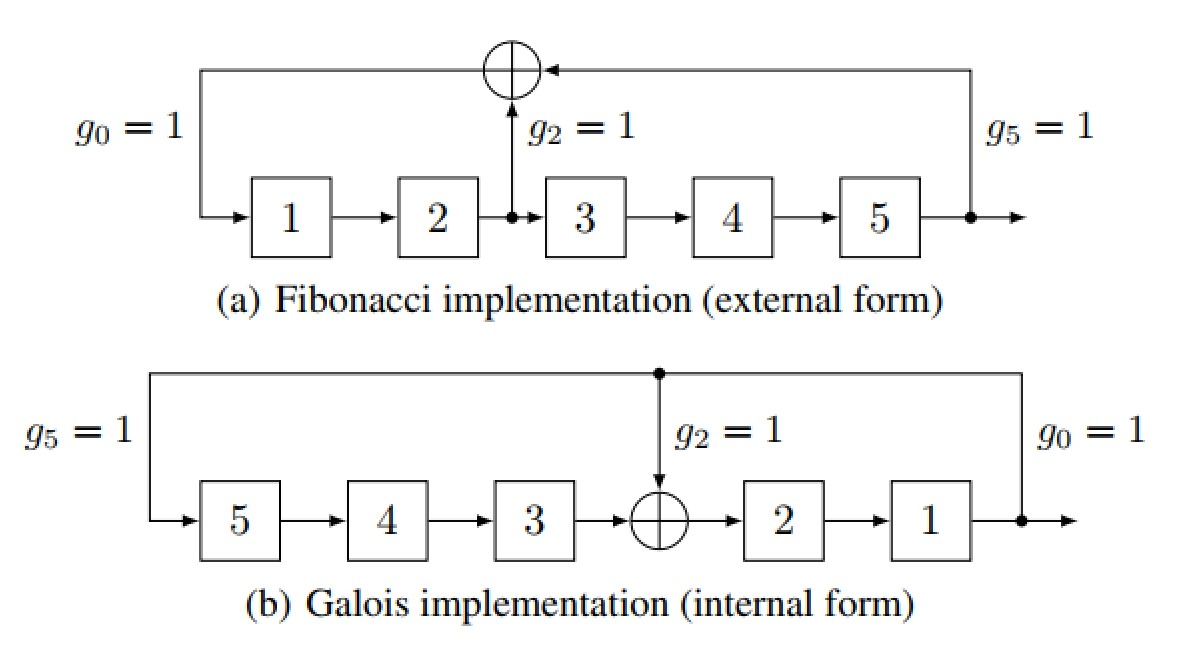
\includegraphics[width=13cm]{images/m-squences.jpg}
  \caption{Example of equivalent forms corresponding to a feedback polynomial of $x^5+x^2+1$.}
  \label{fig:m-squences}
\end{figure}
\subsection{UWB}
A signal is consider as ultra wide band when $\nu$ from \autoref{eq:uwb_condition} is larger than 20\%
\begin{equation}\label{eq:uwb_condition}
\nu=\frac{f_h-f_l}{f_c}=2 \frac{f_h-f_l}{f_h+f_l}
\end{equation}
\begin{itemize}
    \item $f_h$: higher cut off frequency
    \item $f_l$: lower cut off frequency
    \item $f_c$: center frequency
\end{itemize}
